\documentclass[letterpaper]{report}
%\usepackage[utf8]{inputenc}
\usepackage[T1]{fontenc}
\usepackage{RJournal}
\usepackage{amsmath,amssymb,array}
\usepackage{booktabs}

%% load any required packages here

\usepackage[spanish]{babel}
\usepackage{graphicx}

\hypersetup{pdftitle={Agendas científicas sobre desarrollo infantil:
relevamiento y análisis de datos abiertos del CONICET},
            pdfkeywords={Agendas científicas; Desarrollo
infantil; CONICET}}



\hypersetup{pdfauthor=Anónimo}

\newlength{\cslhangindent}
\setlength{\cslhangindent}{1.5em}
\newenvironment{CSLReferences}%
{\setlength{\parindent}{0pt}%
\everypar{\setlength{\hangindent}{\cslhangindent}}\ignorespaces}%
{\par}
%\usepackage[hidelinks]{hyperref}

\urlstyle{same}  % don't use monospace font for urls
\usepackage{color}
\usepackage{fancyvrb}
\newcommand{\VerbBar}{|}
\newcommand{\VERB}{\Verb[commandchars=\\\{\}]}
\DefineVerbatimEnvironment{Highlighting}{Verbatim}{commandchars=\\\{\}} 
% Add ',fontsize=\small' for more characters per line
\usepackage{framed}
\definecolor{shadecolor}{RGB}{248,248,248}
\newenvironment{Shaded}{\begin{snugshade}}{\end{snugshade}}
\newcommand{\AlertTok}[1]{\textcolor[rgb]{0.94,0.16,0.16}{#1}}
\newcommand{\AnnotationTok}[1]{\textcolor[rgb]{0.56,0.35,0.01}{\textbf{\textit{#1}}}}
\newcommand{\AttributeTok}[1]{\textcolor[rgb]{0.77,0.63,0.00}{#1}}
\newcommand{\BaseNTok}[1]{\textcolor[rgb]{0.00,0.00,0.81}{#1}}
\newcommand{\BuiltInTok}[1]{#1}
\newcommand{\CharTok}[1]{\textcolor[rgb]{0.31,0.60,0.02}{#1}}
\newcommand{\CommentTok}[1]{\textcolor[rgb]{0.56,0.35,0.01}{\textit{#1}}}
\newcommand{\CommentVarTok}[1]{\textcolor[rgb]{0.56,0.35,0.01}{\textbf{\textit{#1}}}}
\newcommand{\ConstantTok}[1]{\textcolor[rgb]{0.00,0.00,0.00}{#1}}
\newcommand{\ControlFlowTok}[1]{\textcolor[rgb]{0.13,0.29,0.53}{\textbf{#1}}}
\newcommand{\DataTypeTok}[1]{\textcolor[rgb]{0.13,0.29,0.53}{#1}}
\newcommand{\DecValTok}[1]{\textcolor[rgb]{0.00,0.00,0.81}{#1}}
\newcommand{\DocumentationTok}[1]{\textcolor[rgb]{0.56,0.35,0.01}{\textbf{\textit{#1}}}}
\newcommand{\ErrorTok}[1]{\textcolor[rgb]{0.64,0.00,0.00}{\textbf{#1}}}
\newcommand{\ExtensionTok}[1]{#1}
\newcommand{\FloatTok}[1]{\textcolor[rgb]{0.00,0.00,0.81}{#1}}
\newcommand{\FunctionTok}[1]{\textcolor[rgb]{0.00,0.00,0.00}{#1}}
\newcommand{\ImportTok}[1]{#1}
\newcommand{\InformationTok}[1]{\textcolor[rgb]{0.56,0.35,0.01}{\textbf{\textit{#1}}}}
\newcommand{\KeywordTok}[1]{\textcolor[rgb]{0.13,0.29,0.53}{\textbf{#1}}}
\newcommand{\NormalTok}[1]{#1}
\newcommand{\OperatorTok}[1]{\textcolor[rgb]{0.81,0.36,0.00}{\textbf{#1}}}
\newcommand{\OtherTok}[1]{\textcolor[rgb]{0.56,0.35,0.01}{#1}}
\newcommand{\PreprocessorTok}[1]{\textcolor[rgb]{0.56,0.35,0.01}{\textit{#1}}}
\newcommand{\RegionMarkerTok}[1]{#1}
\newcommand{\SpecialCharTok}[1]{\textcolor[rgb]{0.00,0.00,0.00}{#1}}
\newcommand{\SpecialStringTok}[1]{\textcolor[rgb]{0.31,0.60,0.02}{#1}}
\newcommand{\StringTok}[1]{\textcolor[rgb]{0.31,0.60,0.02}{#1}}
\newcommand{\VariableTok}[1]{\textcolor[rgb]{0.00,0.00,0.00}{#1}}
\newcommand{\VerbatimStringTok}[1]{\textcolor[rgb]{0.31,0.60,0.02}{#1}}
\newcommand{\WarningTok}[1]{\textcolor[rgb]{0.56,0.35,0.01}{\textbf{\textit{#1}}}}

\providecommand{\keywords}[1]{\noindent\textbf{Palabras clave:} #1}
\providecommand{\tightlist}{%
\setlength{\itemsep}{0pt}\setlength{\parskip}{0pt}}



\begin{document}

%% do not edit, for illustration only
\sectionhead{Agendas científicas sobre desarrollo infantil: relevamiento
y análisis de datos abiertos del CONICET}
\year{}

\begin{article}

\title{Agendas científicas sobre desarrollo infantil: relevamiento y
análisis de datos abiertos del CONICET}


\author{Anónimo}

\maketitle


\keywords{ Agendas científicas  -  Desarrollo infantil  -  CONICET }

\section{1. Introducción}\label{introducciuxf3n}

En Argentina, la problemática del desarrollo infantil integral y en
particular de la ``primera infancia'' ganó relevancia en la agenda
política de las últimas décadas a partir de la sanción de leyes y el
despliegue de políticas públicas orientadas a promover el desarrollo de
niños, niñas y adolescentes (NNyA). Ello se produjo en diálogo con
agendas internacionales y regionales que demandaron acciones de los
gobiernos nacionales, provinciales y municipales a partir de la
agudización de los índices de pobreza y desigualdad en NNyA de todo el
mundo. Este periodo coincide con el despliegue de políticas científicas
que apuntaron a una valorización creciente de las áreas de ciencia y
tecnología como herramientas fundamentales para el desarrollo de la
Argentina; y con el posicionamiento discursivo del Estado de orientar la
ciencia hacia la resolución de problemas sociales. Lo dicho se expresó,
en términos concretos, en el aumento progresivo del presupuesto hasta el
año 2015, que se volcó en nuevas infraestructuras, subsidios para
investigación y formación de recursos humanos particularmente a través
del CONICET. En este contexto político de puesta en valor de la ciencia
como instrumento de desarrollo, comenzamos a preguntarnos por su
consonancia con la agenda científica local. Especificamente, nos
preguntamos si la agenda política local en torno al desarrollo infantil
era acompañada por un crecimiento en el financiamiento de proyectos de
investigación científica orientados al tema. Para dar respuesta a este
interrogante, realizamos pedidos de información pública CONICET con el
objetivo de analizar el comportamiento de las becas e ingresos otorgados
por organismo en el periodo 2010-2020 a candidatos y candidatas con
temas vinculados al desarrollo de NNyA. Nos propusimos analizar, en
términos cuantitativos, si la creciente relevancia pública otorgada a
esta problemática se vio acompañada de un aumento en el ingreso de
becarios e investigadores al CONICET interesados en temáticas afines. En
el año 2024, realizamos una primera publicación de dichos análisis en un
artículo científico y pusimos a disposición los datos tal como fueron
procesados en un repositorio de Github. Los resultados obtenidos
mostraron la relevancia pública otorgada al desarrollo infantil durante
el período analizado a partir del interés del Estado por financiar
proyectos sobre estos temas. A partir de ello, decidimos avanzar hacia
la creación de una aplicación web que permitiera el acceso y la
exploración de los datos recolectados para colegas tanto del ámbito
académico como del ámbito profesional que estuvieran interesados/as en
comprender la inserción de estas temáticas a lo largo de la Argentina.
Por un lado, consideramos que este tipo de herramienta podría ser
relevante para la construcción y fortalecimiento de redes entre equipos
profesionales y/o de investigación que tengan temáticas, intereses y
objetivos en común. A la vez, creemos que la disponibilidad y
accesibilidad de estos datos es importante para la toma de decisiones,
resolución de problemas e innovación científico tecnológica. En
concreto, pensamos en la construcción de una herramienta que permita
analizar las agendas de investigación en la Argentina y tomar decisiones
basadas tanto en los datos disponibles como en los objetivos de los
organismos, institutos, grupos de investigación e individuos.

\section{2. Obtención de los datos}\label{obtenciuxf3n-de-los-datos}

Los datos requeridos para los análisis fueron solicitados a CONICET a
través de la plataforma de Trámites a Distancia (TAD,
https://tramitesadistancia.gob.ar) bajo la modalidad de Acceso a la
Información Pública. En particular, se solicitó información sobre las
becas otorgadas e ingresos a CIC entre los años 2010 y 2020 para Temas
Generales y Temas Estratégicos. Para identificar aquellos proyectos
asociados al estudio del desarrollo de NNyA, se consensuaron una serie
de criterios de inclusión basados en el análisis del título, resumen y
palabras clave de los proyectos. La selección de los proyectos fue
realizada de forma manual por cuatro asistentes de investigación.

\section{3. Implementación de una Shiny para el acceso a los
datos}\label{implementaciuxf3n-de-una-shiny-para-el-acceso-a-los-datos}

Con el objetivo de disponibilizar los datos al público tanto académico
como profesional, se desarrolló una aplicación web interactiva (Figura
1) que permite visualizar la distribución de los distintos proyectos de
investigación sobre desarrollo de NNyA de acuerdo al año de la
convocatoria (de 2010 a 2020), por el tipo de ingreso (beca doctoral,
beca postdoctoral, o CIC), el tipo de modalidad (temas generales o
específicos), la comisión evaluadora, y la región del país donde está
radicado el ingreso. Por otro lado, la shiny incluye un mapa interactivo
que, al día de hoy, permite visualizar la distribución geográfica de los
distintos proyectos y explorar el cambio en dicha distribución a lo
largo de los años. Finalmente, se pone a disposición una tabla
interactiva que permite filtrar los distintos proyectos a partir de las
categorías propuestas.

\begin{figure}
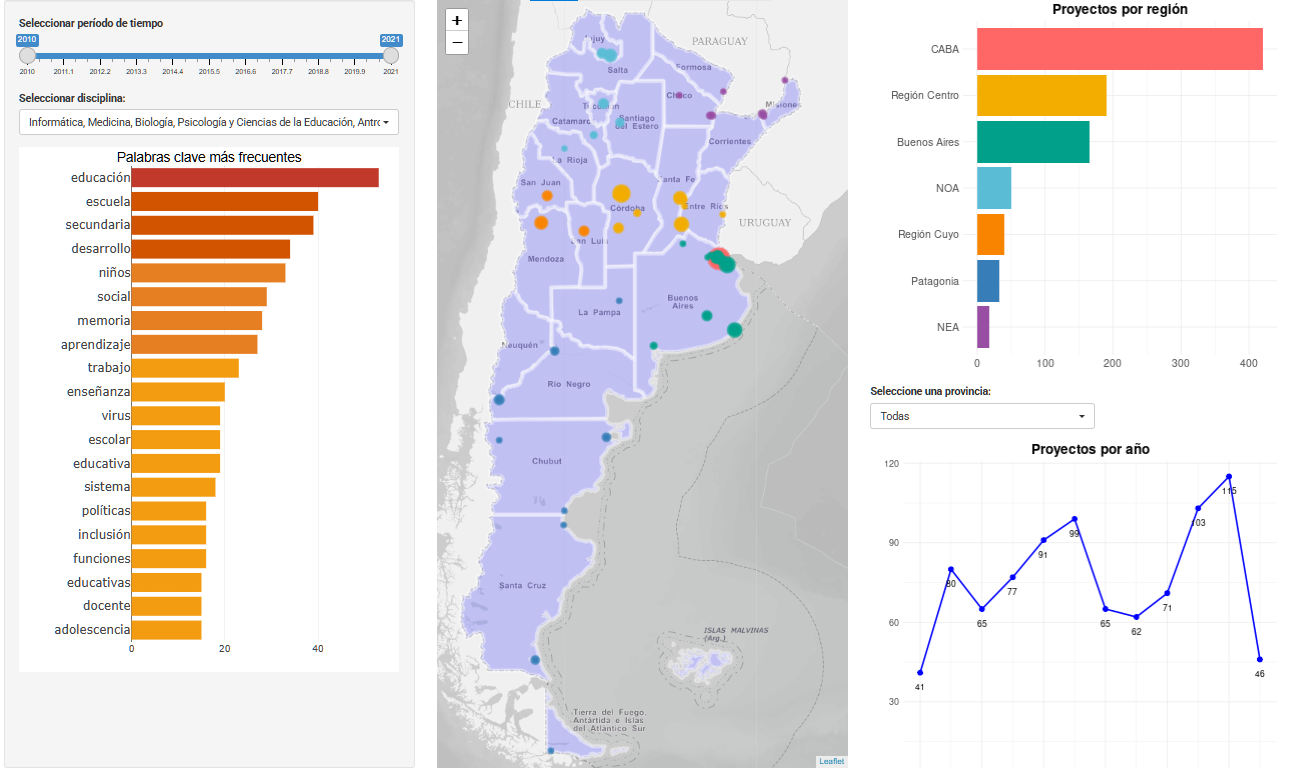
\includegraphics[width=1\linewidth]{Figura1} \caption{Panel central de la Aplicación Shiny}\label{fig:Figura-1}
\end{figure}

Todos los análisis se realizaron mediante el lenguaje R versión 4.2.1
\citep{R-base}, en Rstudio \citep{R-studio}. Los principales paquetes
utilizados fueron dplyr \citep{R-dplyr}, ggplot2 \citep{R-ggplot2},
leaflet \citep{R-leaflet}, y geoAr \citep{R-geoAr}.

\section{4. Direcciones futuras}\label{direcciones-futuras}

Lo realizado hasta ahora permitió implementar una herramienta accesible
para cualquier profesional, docente o investigador que esté interesado
en conocer qué grupos investigan qué temas en la Argentina. En el futuro
inmediato, esperamos poder incorporar métodos de aprendizaje automático
que identifiquen los distintos tópicos presentes en las agendas de
investigación y su prevalencia a lo largo de los años y de las distintas
regiones del país. En el mediano plazo, también esperamos poder
construir una infraestructura capaz de incorporar nuevos datos
(e.g.~provenientes de nuevos ingresos de becarios e investigadores) de
forma rápida y con la menor intervención humana posible. Finalmente, en
el largo plazo esperamos poder generalizar esta herramienta hacia una
aplicación o sistema de monitoreo que permita el análisis y la
exploración de agendas de investigación de diversas áreas y temáticas
con el fin de que sirva al Estado y a sus diversos organismos de Ciencia
y Tecnología para tomar decisiones y establecer agendas de
investigación.

\bibliography{latinr_bibliography}




\end{article}
\end{document}
